\chapter{Average runtime of solvers by problem type and sizes}\label{appendix:timesizegraph}

\section{NAE3SAT}
\autoref{time-nae3sat-size} shows the average runtime taken for NAE3SAT problems.
\begin{figure}[!htb]
    \centering
    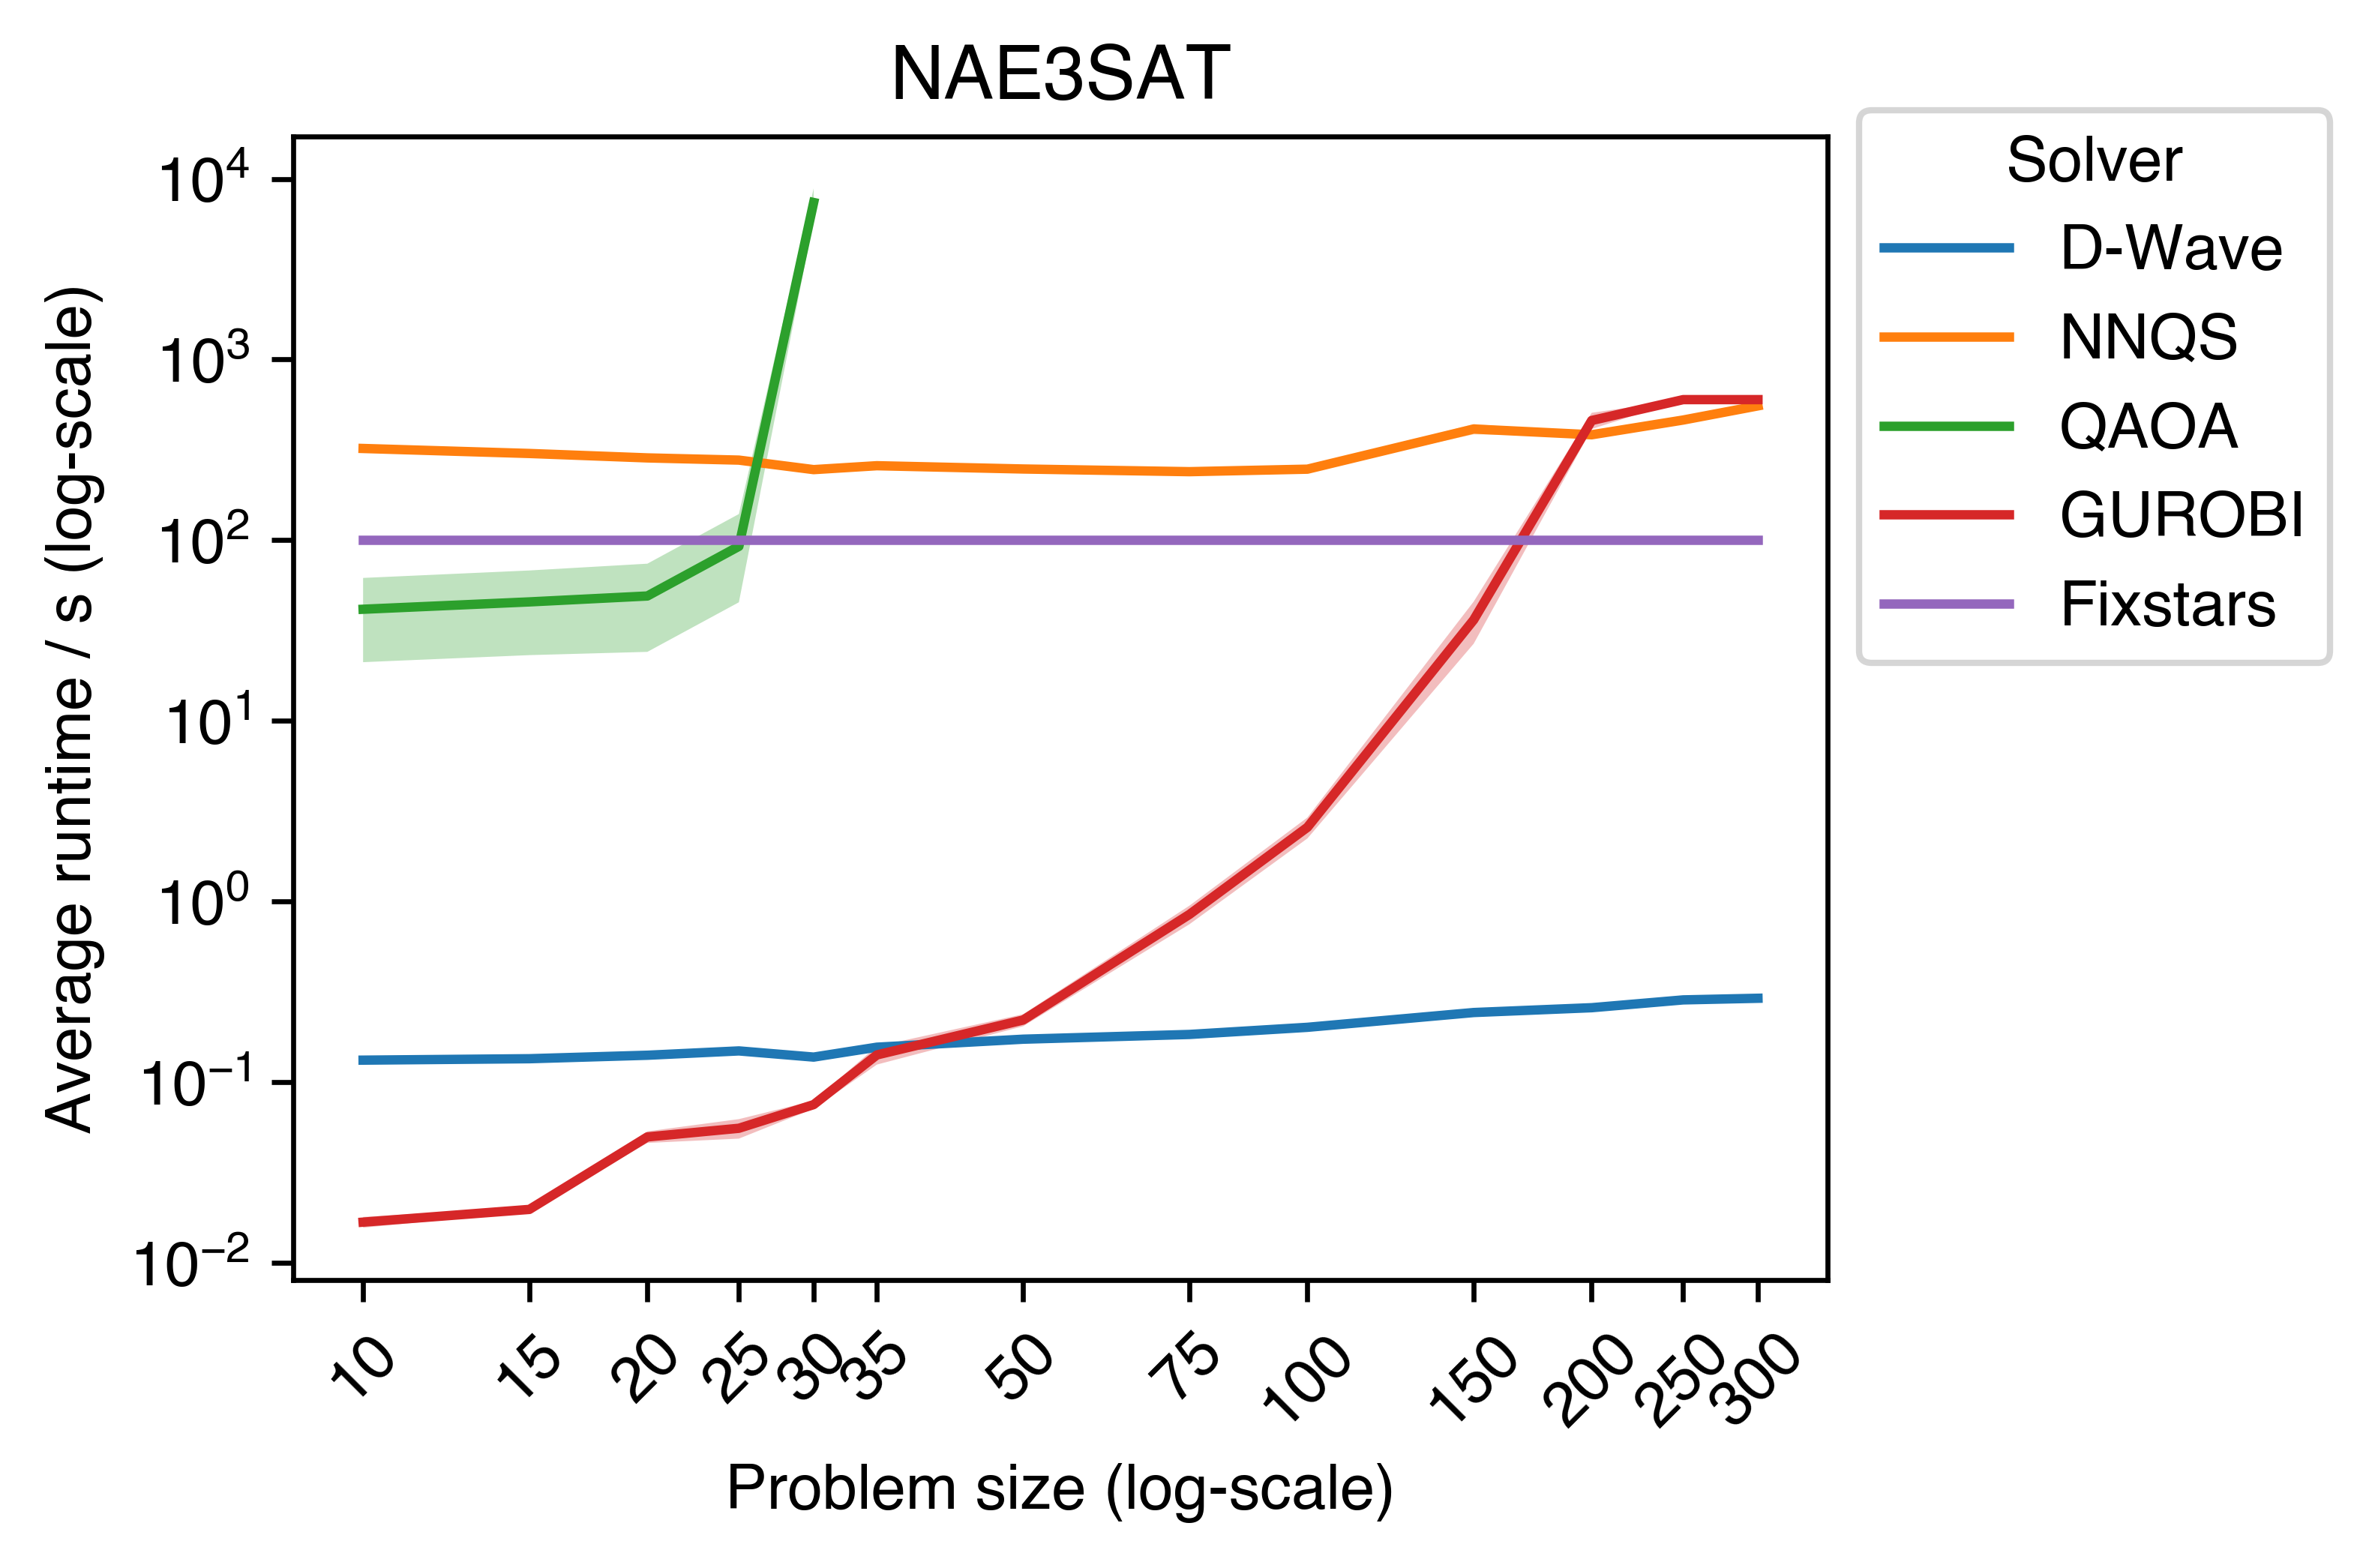
\includegraphics[width=0.6\textwidth]{images/nae3sat_all_time_size.png}
    \caption{Average runtime taken by different solvers for NAE3SAT by problem size}
    \label{time-nae3sat-size}
\end{figure}

\section{Max-cut}
\autoref{time-maxcut-size} shows the average runtime taken for max-cut problems.
\begin{figure}[!htb]
    \centering
    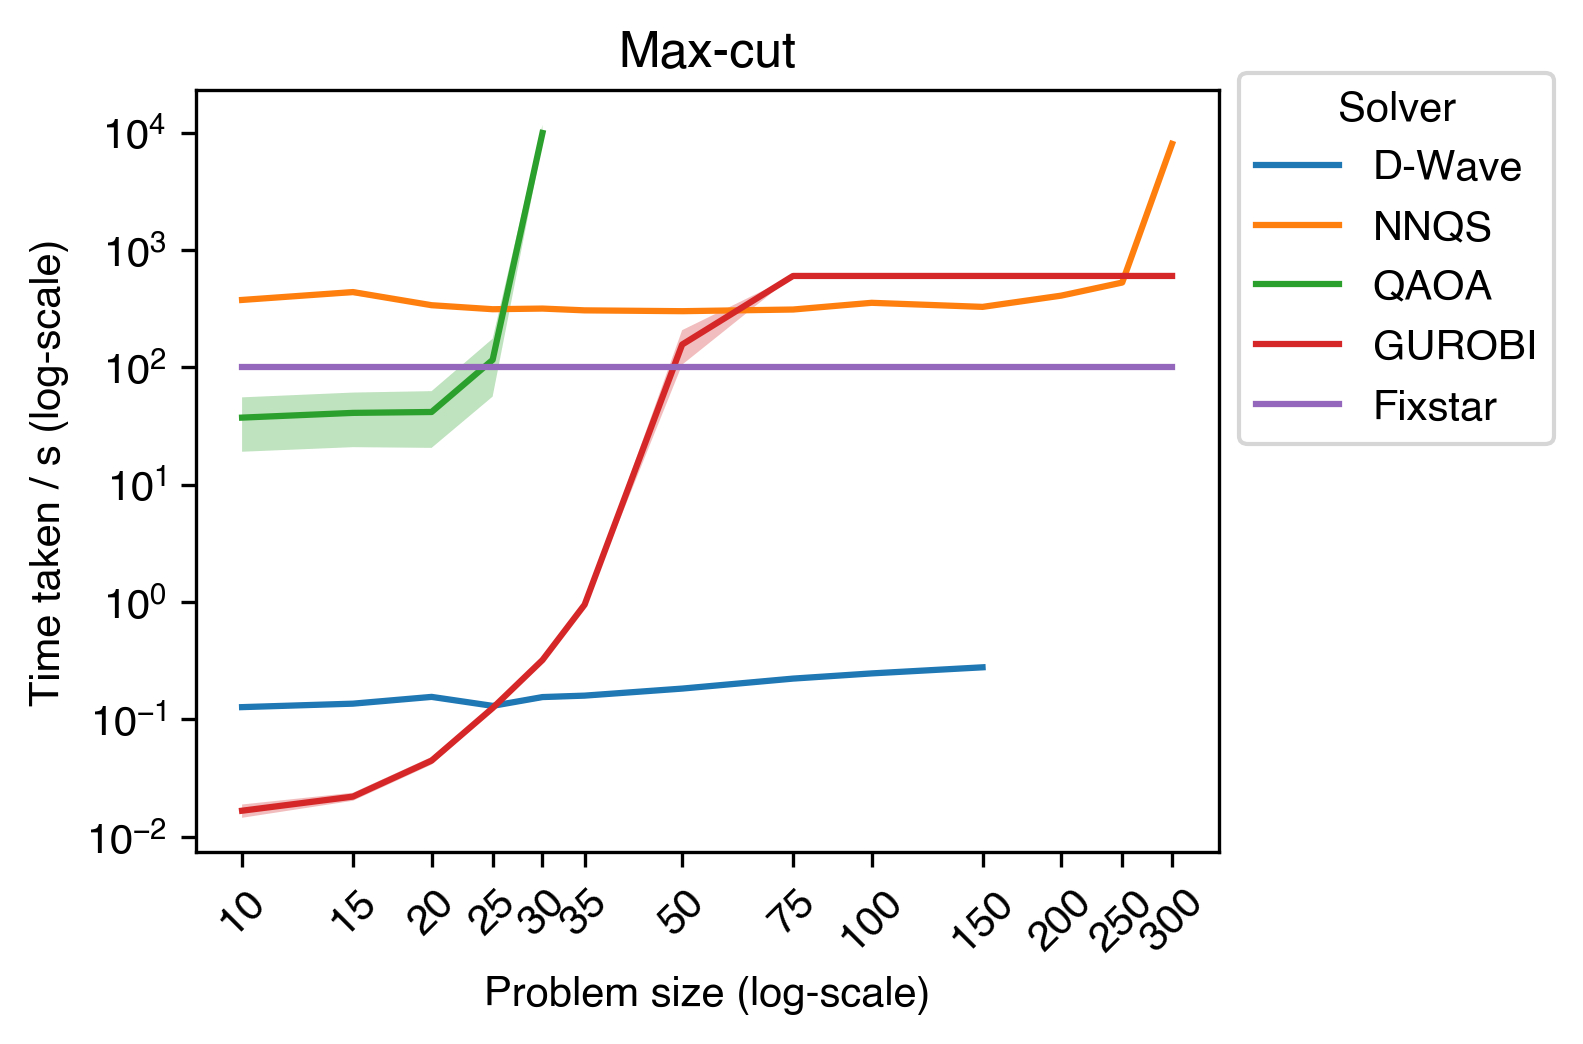
\includegraphics[width=0.6\textwidth]{images/maxcut_all_time_size.png}
    \caption{Average runtime taken by different solvers for max-cut by problem size}\label{time-maxcut-size}
\end{figure}

\section{SK model}
\autoref{time-skmodel-size} shows the average runtime taken for SK model problems.
\begin{figure}[!htb]
    \centering
    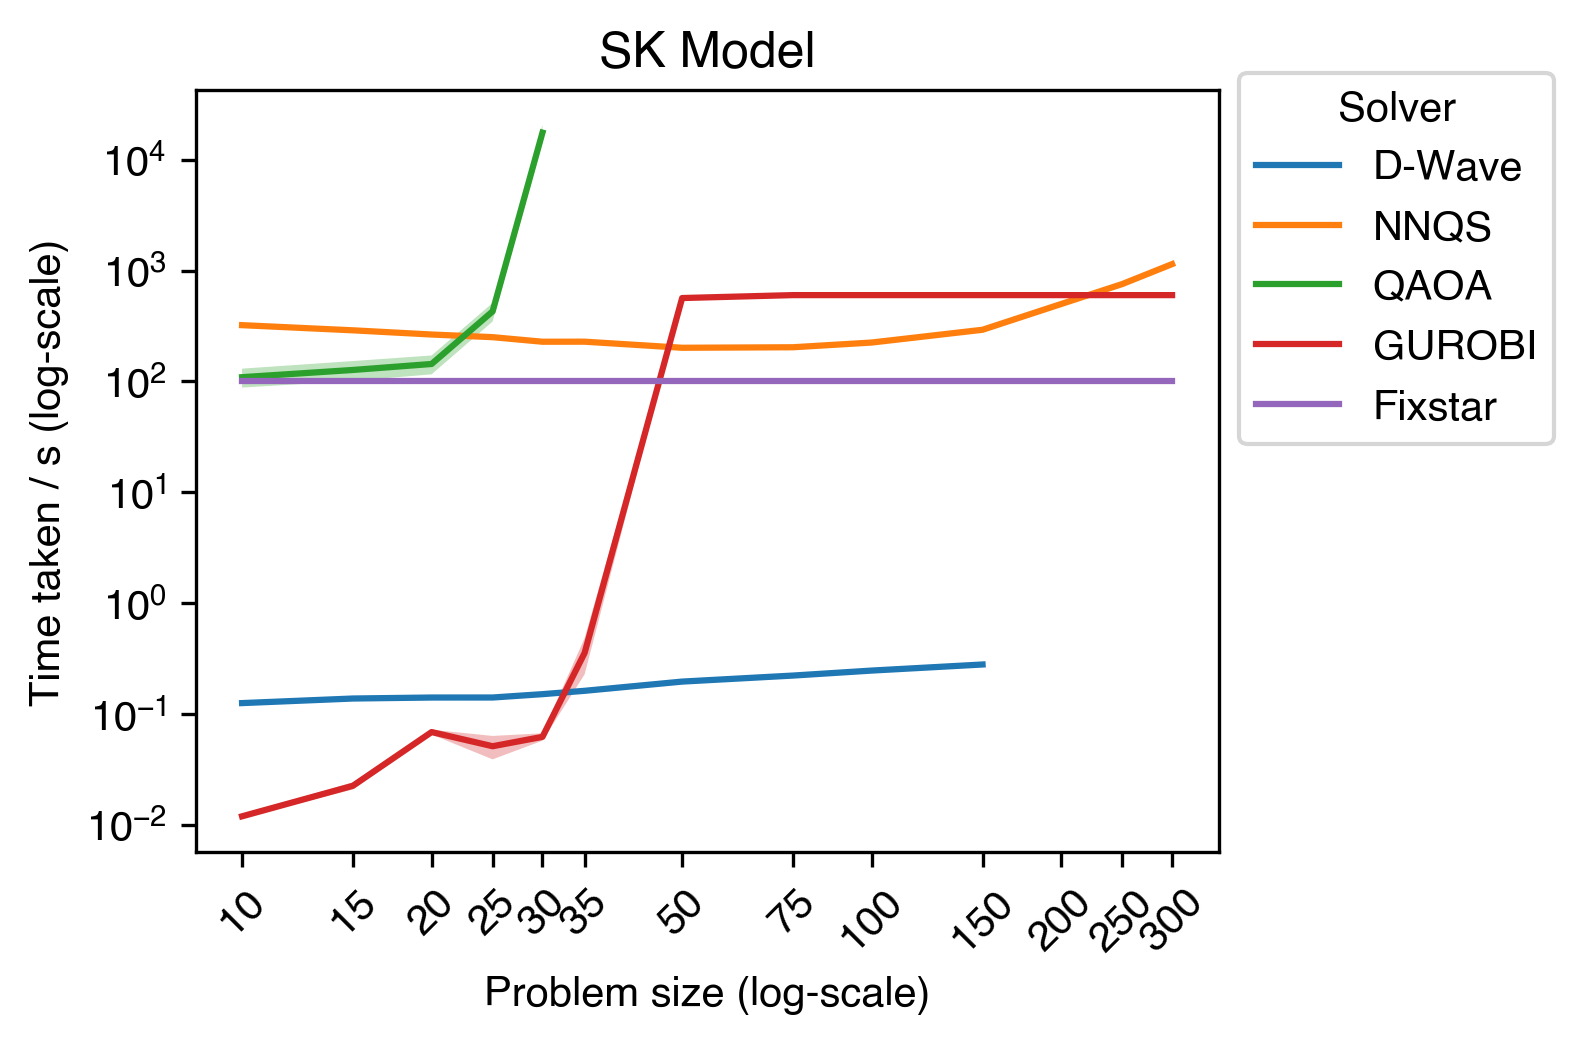
\includegraphics[width=0.6\textwidth]{images/skmodel_all_time_size.png}
    \caption{Average runtime taken by different solvers for SK model by problem size}    \label{time-skmodel-size}
\end{figure}